\section{Analyse}\label{kapitel4}
\subsection{Einleitung}
\subsubsection{Zweck der Anwendung}
Die App soll es ermöglichen, einen Lauf mitzuschneiden, um ihn anschließend an eine Gruppe von Freunden zu veröffentlichen. Diesen ist es dann möglich, mit ihren Freunden zu laufen bzw. gegen diese anzutreten. Läufe sollen regelmäßig (z.B. einmal pro Woche) stattfinden, um ein regelmäßiges zurückkehren zu unserer App und dem Sport zu gewährleisten. Um Läufe vergleichbar zu machen sollen Höhendaten berücksichtigt werden, um Läufern auf bergigen Strecken, die anstrengender zu Laufen sind eine faire Chance zu geben.

Während des Laufes soll ein direkter Vergleich zur Konkurrenz möglich sein. Dies geschieht durch die Einblendung sogenannter Geister, also die Darstellung des Fortschritts der bereits gelaufenen Gegner im Vergleich zum eigenen. Auch während des Laufens werden Nutzer so angetrieben, ihr Bestes zu geben.

Um die Funktionalität zu gewährleisten sind das Schreiben einer Android-App und das Aufzetzen eines Webserver nötig, der als zentraler Datenspeicher agiert und die verschiedenen Nutzer verbindet.
\subsubsection{Projektumfang}
Ziel der App ist es nicht, wie andere Fitness-, bzw. Joggingapps umfangreiche Statistiken anzubieten. Vielmehr konzentrieren wir uns in der Arbeit darauf, Gamification zu nutzen und durch den direkt ersichtlichen Wettbewerb die Nutzer anzuspornen. Statt ausführlicher Statistiken soll ein GPX-Export ermöglicht werden, damit Nutzer ihre Läufe später in beliebiger Software importieren und auswerten können. So ist unsere App keine Konkurrenz zu vielen etablierten Fitnessportalen, sondern lässt sich als Ergänzung nutzen.

Weiterhin ist es keine Anforderung, ein vollständiges Social Network mit Privat- und Gruppenunterhaltungen bereitzustellen. Diese Funktionalität kann in späteren Versionen der App durchaus implementiert werden, ist aber nicht Hauptaspekt der Studienarbeit. Wichtig ist dagegen, Funktionalität anzubieten um Gruppen zu verwalten, also Nutzer hinzuzufügen und zu löschen.

Die Benutzeroberfläche der App soll ansprechend gestaltet werden, dennoch ist sie nicht Hauptaspekt der Arbeit, da dies in Kombination mit der übrigen Funktionalität den Rahmen einer Studienarbeit sprengen würde. Insbesondere der Bildschirm während des Laufens soll hierbei ein Wiedererkennungsmerkmal darstellen. In der Version, die während der Studienarbeit geschrieben wird, soll ersichtlich werden, wie eine spätere, professionell gestaltete Oberfläche aussehen könnte.

Wir können keinen direkten Einfluss auf die Skalierbarkeit und Verfügbarkeit des Webservers nehmen, da dieser auf einer virtuellen Maschine der DHBW läuft. Dennoch sollte der Webserver aus programmatischer Sicht gewissen Performanceanforderungen genügen.
\subsection{Funktionale Anforderungen}
\subsubsection{Webserver}
Der Webserver stellt dem Klienten eine Schnittstelle bereit, um Nutzer, Gruppen und Läufe zu verwalten. Er muss dabei folgende Funktionale Anforderungen erfüllen:
\begin{itemize}
\item Authentifizierung durch Nutzername und Passwort
\item Erstellen und Herausgeben eines Authentifizierungstokens bei Erfolg
\item Authentifizierung durch das Authentifizierungstoken, Zuordnung zum jeweiligen Nutzer
\item Erstellen und Löschen von Nutzern
\item Ausgabe und Modifikation von Nutzerdaten
\item Erstellen und Löschen von Gruppen
\item Ausgabe und Modifikation von Gruppendaten
\item Hinzufügen und Entfernen von Nutzern zu Gruppen
\item Unterscheidung von Gruppenadministratoren und Nutzern
\item Einladen von Nutzern in Gruppen
\item Annehmen und Ablehnen von Einladungen
\item Verwaltung regelmäßiger Stichtage zur Laufauswertung
\item Erstellen und Ausgeben von Läufen, abhängig von Nutzer und Gruppe
\item Ausgabe von Kacheln mit Höhendaten
\end{itemize}
\subsubsection{Android App}
Die Android App muss folgende Funktionalität erfüllen:
\begin{itemize}
\item Anmeldung beim Webserver mit Nutzername und Passwort
\item Speicherung von Anmeldedaten
\item Speicherung des Authentifizierungstokens
\item Authentifizierung beim Webserver mit Authentifizierungstoken
\item Registrierung beim Webserver
\item Abmeldung inklusive Entfernung von Token und Anmeldedaten
\item Anzeigen einer Übersichte aller Gruppen
\item Erstellen von neuen Gruppen
\item Anzeigen einer Übersicht aller Nutzer und aktuellen Läufe einer Gruppe, inklusiver aktueller Platzierung
\item Einladen von bereits vorhandenen Nutzern in eine Gruppe
\item Einladen von appfremden Nutzern in eine Gruppe
\item Löschen von Nutzern aus einer Gruppe
\item Aufzeichnung von Läufen und Übergabe an den Server
\item Exportieren von Läufen im GPX Format
\item Darstellung des Lauffortschritts und Anzeige von Geistern
\item Darstellung einer Statistikseite am Ende von Läufen
\end{itemize}
\subsection{Nichtfunktionale Anforderungen}
\subsubsection{Performanz}
Sowohl die App als auch der Server müssen so konzipiert werden, dass schnelle Reaktionszeiten möglich sind. Ladezeiten sollten für den Nutzer minimiert werden. Insbesondere muss eine Einfrieren der Nutzeroberfläche vermieden werden, längere Berechnungen oder Downloads sollen im Hintergrund ablaufen.

Versendete Datenmengen sollten minimiert werden, da die Verbindungsgeschwindigkeit und -verfügbarkeit gerade während den Läufen nicht garantiert werden kann.
\subsubsection{Usability}
Die App muss einfach zu bedienen sein. Wir richten uns allgemein an Sportler und Sportinteressierte. Außer grundlegenden Kenntnissen zur Nutzung von Android-Apps können wir keine Annahmen zu den technischen Fähigkeiten des Nutzers machen.

Teile der App sind für die Nutzung beim Joggen. Auch hierbei muss es dem Nutzer möglich sein relevante Informationen zu erkennen und sicher mit der App zu interagieren.
\subsubsection{Sicherheit}
Um Nutzer am Server zu authentifizieren ist eine Nutzername/Passwort-Vergabe notwendig. Sie dient zum einen zum Wiedererkennen einzelner Nutzer, als auch um unbefugte Zugriffe auf den Server zu verhindern. Um das Passwort des Nutzers und seine persönlichen Daten zu sichern, müssen diese verschlüsselt gespeichert und versendet werden.

Außerdem muss die Sicherheit des Gerätes zu jedem Zeitpunkt gewährleistet sein, d.h. die Einschleusung über die App von Schadcode darf nicht möglich sein.
\subsection{Use Cases}
\subsubsection{Diagramme}
\begin {figure}[!hb]\label{fig:usecase_login}
\centering
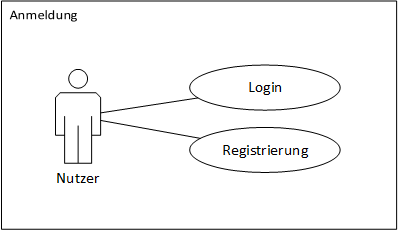
\includegraphics[width=\textwidth]{abb/usecase_login}
\caption{Use Cases der Login Aktivität}
\end{figure}
Während ein Appnutzer ausgeloggt ist, soll ihm keinerlei Funktionalität der App zur Verfügung stehen. Er hat hier also nur die Möglichkeit sich anzumelden oder neu zu registrieren.
\begin {figure}[!hb]\label{fig:usecase_main}
\centering
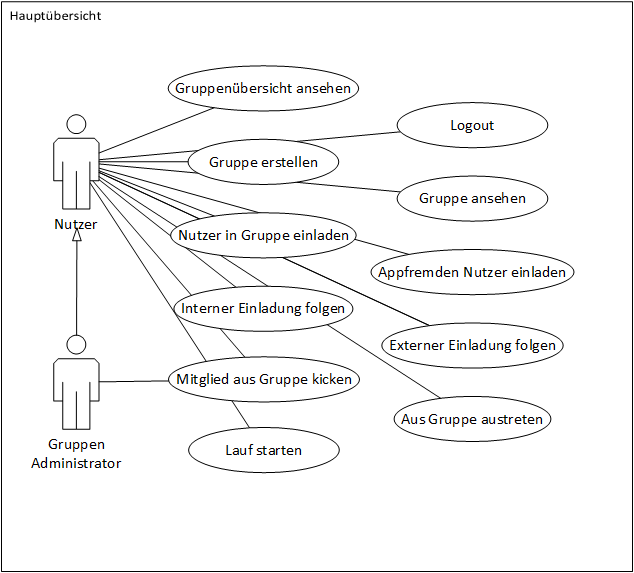
\includegraphics[width=\textwidth]{abb/usecase_main}
\caption{Use Cases der Hauptaktivität}
\end{figure}
Ist der Nutzer eingeloggt und befindet sich nicht in einem Lauf, stehen ihm verschiedene Aktionen zur Verfügung. Er kann hierbei Gruppen verwalten, seine aktuellen Platzierungen ansehen und Läufe starten. Während des Laufens ist diese Funktionalität nicht von Bedeutung, da sich Nutzer hier auf den Sport und sich selbst konzentrieren müssen.
\begin {figure}[!hb]\label{fig:usecase_run}
\centering
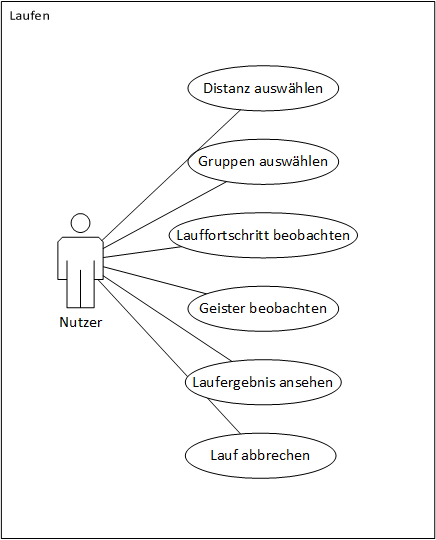
\includegraphics[width=\textwidth]{abb/usecase_run}
\caption{Use Cases der Laufaktivität}
\end{figure}
Soll ein neuer Lauf gestartet werden, muss zunächst die gewünschte Distanz gewählt werden. Danach kann ein Nutzer auswählen, in welchen Gruppen er mit seiner Endzeit antreten möchte und welche Geister angezeigt werden sollen. Die Auswahl einer Gruppe ist hierbei nicht unbedingt notwendig, man kann auch ohne Geister Läufe 
aufzeichnen.
\subsubsection{Beschreibung}
\begin{tabular}{|p{0.2\textwidth}|p{0.8\textwidth}|}
\hline
\textbf{Use Case} & \textbf{Login}  \\ \hline
Aktoren &  Ein Nutzer \\ \hline
Ziel &  Der Nutzer will Zugriff auf die App und seine Daten bekommen \\ \hline
Bedingungen &  Der Nutzer besitzt ein Konto \\ \hline
Beschreibung &  Der Nutzer gibt Name und Passwort an und klickt auf einen Login Button. Die Daten werden an den Server übergeben und von diesem überprüft \\ \hline
Erfolg & Der Server gibt ein Authentifizierungstoken zurück, dass von der App für spätere Netzwerkanfragen gespeichert wird. Die App wechselt zur Hauptansicht  \\ \hline
Misserfolg & Die App zeigt eine Fehlermeldung, die dem Nutzer hilft, sich bei einem erneuten Versuch erfolgreich anzumelden \\ \hline
\hline \end{tabular}
\begin{tabular}{|p{0.2\textwidth}|p{0.8\textwidth}|}
\hline
\textbf{Use Case} & \textbf{Registrierung} \\ \hline
Aktoren &  Ein Nutzer \\  \hline
Ziel &  Der Nutzer will ein neues Konto anlegen, um Zugriff auf die App zu bekommen \\ \hline
Bedingungen &  Keine \\ \hline
Beschreibung &  Der Nutzer gibt seinen gewünschten Nutzernamen, Email und Passwort an und klickt auf einen. Die Daten werden an den Server übergeben und von diesem überprüft und gespeichert \\ \hline
Erfolg & Ein neues Nutzerkonto wird erstellt. Der Nutzer wird eingeloggt und hat Zugriff auf alle Funktionen der App \\ \hline
Misserfolg & Die App zeigt eine Fehlermeldung, die dem Nutzer hilft, sich bei einem erneuten Versuch erfolgreich zu registrieren \\ \hline
\hline \end{tabular}
\begin{tabular}{|p{0.2\textwidth}|p{0.8\textwidth}|}
\hline
\textbf{Use Case} & \textbf{Gruppenübersicht ansehen} \\ \hline
Aktoren &  Ein Nutzer \\ \hline
Ziel &  Der Nutzer will einen Überblick über alle Gruppen bekommen, in denen er sich befindet. \\ \hline
Bedingungen &  Der Nutzer ist angemeldet und befindet sich in der Hauptaktivität\\ \hline
Beschreibung &  Es wird eine Liste aller Gruppen des Nutzers angezeigt. Zusätzlich gibt es Menüpunkte für das Anlegen neuer Gruppen und dem Folgen interner Einladungen \\ \hline
Erfolg & Die Gruppenübersicht wird angezeigt \\ \hline
Misserfolg & Der Nutzer wird abgemeldet, falls eine Authentifizierung nicht möglich ist \\ \hline
\hline \end{tabular}
\begin{tabular}{|p{0.2\textwidth}|p{0.8\textwidth}|}
\hline
\textbf{Use Case} & \textbf{Lauf starten} \\ \hline
Aktoren &  Ein Nutzer \\ \hline
Ziel &  Der Nutzer will einen neuen Lauf starten \\ \hline
Bedingungen &  Der Nutzer ist angemeldet und befindet sich in der Hauptaktivität. Der Lokalisierungsdienst ist aktiviert \\ \hline
Beschreibung &  Es wird eine Auswahl aller möglichen Distanzen und zugehörigen Gruppen angezeigt\\ \hline
Erfolg & Der Dialog zum Starten eines Laufs wird angezeigt \\ \hline
Misserfolg & Der Nutzer wird aufgefordert, den Lokalisierungsdienst zu starten \\ \hline
\hline \end{tabular}
\begin{tabular}{|p{0.2\textwidth}|p{0.8\textwidth}|}
\hline
\textbf{Use Case} & \textbf{Gruppe erstellen} \\ \hline
Aktoren &  Ein Nutzer \\ \hline
Ziel &  Eine neue Gruppe soll auf dem Server erstellt werden. Der Nutzer soll sich darin befinden \\ \hline
Bedingungen &  Der Nutzer ist angemeldet und befindet sich in der Hauptaktivität. \\ \hline
Beschreibung &  Der Nutzer gibt Gruppenname und die regelmäßig zu laufende Distanz an \\ \hline
Erfolg & Die Gruppe wird erstellt und dem Nutzer angezeigt \\ \hline
Misserfolg & Der Nutzer wird abgemeldet, falls eine Authentifizierung nicht möglich ist \\ \hline
\hline \end{tabular}
\begin{tabular}{|p{0.2\textwidth}|p{0.8\textwidth}|}
\hline
\textbf{Use Case} & \textbf{Gruppe ansehen} \\ \hline
Aktoren &  Ein Nutzer \\ \hline
Ziel &  Der Nutzer möchte die Gruppenmitglieder und ihre Platzierungen ansehen oder die Gruppe verwalten \\ \hline
Bedingungen &  Der Nutzer ist angemeldet und befindet sich in der Hauptaktivität. Er ist Mitglied einer Gruppe \\ \hline
Beschreibung & Die Mitglieder der Gruppe werden in aktueller Reihenfolge angezeigt. Es gibt die Möglichkeit, die Gruppe zu verwalten. Der nächste Stichtag für die Laufauswertung wird angezeigt \\ \hline
Erfolg & Die Gruppenansicht wird angezeigt \\ \hline
Misserfolg & Der Nutzer wird abgemeldet, falls eine Authentifizierung nicht möglich ist \\ \hline
\hline \end{tabular}
\begin{tabular}{|p{0.2\textwidth}|p{0.8\textwidth}|}
\hline
\textbf{Use Case} & \textbf{Nutzer in Gruppe einladen} \\ \hline
Aktoren &  Ein Nutzer \\ \hline
Ziel &  Der Nutzer möchte ein neues Gruppenmitglied einladen \\ \hline
Bedingungen &  Der Nutzer ist angemeldet und befindet sich in der Hauptaktivität. Er ist Mitglied einer Gruppe \\ \hline
Beschreibung & Der Nutzer gibt den gewünschten Nutzernamen in eine Suchmaske ein. Ergebnisse werden ihm angezeigt. Der Nutzer wählt ein Ergebnis aus, woraufhin in der Datenbank eine neue Einladung erstellt wird, die bein Eingeladenen angezeigt wird \\ \hline
Erfolg & Die Einladung wird erstellt und dem Eingeladenen angezeigt \\ \hline
Misserfolg & Kann der gesuchte Name nicht gefunden werden, wird dem Nutzer dies angezeigt. Der Nutzer wird abgemeldet, falls eine Authentifizierung nicht möglich ist \\ \hline
\hline \end{tabular}
\begin{tabular}{|p{0.2\textwidth}|p{0.8\textwidth}|}
\hline
\textbf{Use Case} & \textbf{Appfremden Nutzer einladen} \\ \hline
Aktoren &  Ein Nutzer \\ \hline
Ziel &  Der Nutzer möchte ein neues Gruppenmitglied einladen, dessen Nutzernamen er nicht kennt, oder der die App nicht installiert hat \\ \hline
Bedingungen &  Der Nutzer ist angemeldet und befindet sich in der Hauptaktivität. Er ist Mitglied einer Gruppe \\ \hline
Beschreibung & Der Nutzer betätigt die Teilen Funktion der App. Der Server erstellt eine PIN, die der Gruppe zugeordnet ist. Die PIN kann zusammen mit der Aufforderung, Gh0strunner zu installieren, über beliebige andere Apps versendet werden \\ \hline
Erfolg & Eine PIN wird erstellt und dem Eingeladenen gesendet \\ \hline
Misserfolg & Der Nutzer wird abgemeldet,falls eine Authentifizierung nicht möglich ist \\ \hline
\hline \end{tabular}
\begin{tabular}{|p{0.2\textwidth}|p{0.8\textwidth}|}
\hline
\textbf{Use Case} & \textbf{Interner Einladung folgen} \\ \hline
Aktoren &  Ein Nutzer \\ \hline
Ziel &  Der Nutzer möchte Mitglied einer Gruppe werden, in die er eingeladen wurde \\ \hline
Bedingungen &  Der Nutzer ist angemeldet und befindet sich in der Gruppenübersicht. Er wurde von einem anderen Nutzer eingeladen \\ \hline
Beschreibung & In der Gruppenübersicht wird dem Nutzer eine sonst unsichtbare Option angezeigt, einer neuen Gruppe beizutreten. Akzeptiert der Nutzer die Einladung wird er der Gruppe hinzugefügt \\ \hline
Erfolg & Der Nutzer wird Mitglied der Gruppe \\ \hline
Misserfolg & Der Nutzer wird abgemeldet, falls eine Authentifizierung nicht möglich ist. Er ist kein Mitglied der Gruppe \\ \hline
\hline \end{tabular}
\begin{tabular}{|p{0.2\textwidth}|p{0.8\textwidth}|}
\hline
\textbf{Use Case} & \textbf{Externer Einladung folgen} \\ \hline
Aktoren &  Ein Nutzer \\ \hline
Ziel &  Der Nutzer möchte Mitglied einer Gruppe werden, in die er mit einer PIN eingeladen wurde \\ \hline
Bedingungen &  Der Nutzer ist angemeldet und befindet sich in der Hauptaktivität. Er wurde von einem anderen Nutzer eingeladen \\ \hline
Beschreibung & Der Nutzer gibt eine PIN ein. Diese wird vom Server überprüft und der Nutzer wird zur korrespondierenden Gruppe eingeladen \\ \hline
Erfolg & Der Nutzer wird Mitglied der Gruppe \\ \hline
Misserfolg & Ist die PIN abgelaufen oder ungültig, wird dies dem Nutzer angezeigt. Er wird abgemeldet, falls eine Authentifizierung fehlschlägt. \\ \hline
\hline \end{tabular}
\begin{tabular}{|p{0.2\textwidth}|p{0.8\textwidth}|}
\hline
\textbf{Use Case} & \textbf{Aus Gruppe austreten} \\ \hline
Aktoren &  Ein Nutzer \\ \hline
Ziel &  Der Nutzer möchte Mitglied aus einer Gruppe austreten\\ \hline
Bedingungen &  Der Nutzer ist angemeldet und befindet sich in der Gruppenansicht. Er ist Mitglied einer Gruppe \\ \hline
Beschreibung & Der Nutzer betätigt einen Button. Er wird daraufhin aus der Gruppe entfernt \\ \hline
Erfolg & Der Nutzer ist kein Mitglied der Gruppe mehr \\ \hline
Misserfolg & Der Nutzer wird abgemeldet, falls eine Authentifizierung fehlschlägt. \\ \hline
\hline \end{tabular}
\begin{tabular}{|p{0.2\textwidth}|p{0.8\textwidth}|}
\hline
\textbf{Use Case} & \textbf{Mitglied aus Gruppe Kicken} \\ \hline
Aktoren &  Ein Gruppenadministrator \\ \hline
Ziel &  Der Nutzer möchte Mitglied ein Mitglied aus einer Gruppe entfernen \\ \hline
Bedingungen &  Der Nutzer ist angemeldet und befindet sich in der Gruppenansicht. Er ist Administrator der Gruppe \\ \hline
Beschreibung & Der Nutzer betätigt einen Button. Das zu entfernende Mitglied wird daraufhin aus der Gruppe gelöscht \\ \hline
Erfolg & Das Mitglied ist kein Mitglied der Gruppe mehr \\ \hline
Misserfolg & Das Mitglied wird nicht gelöscht, falls der Nutzer kein Gruppenadministrator ist. Der Nutzer wird abgemeldet, falls eine Authentifizierung fehlschlägt. \\ \hline
\hline \end{tabular}
\begin{tabular}{|p{0.2\textwidth}|p{0.8\textwidth}|}
\hline
\textbf{Use Case} & \textbf{Logout} \\ \hline
Aktoren &  Ein Nutzer \\ \hline
Ziel &  Der Nutzer möchte sich abmelden \\ \hline
Bedingungen &  Der Nutzer ist angemeldet und befindet sich in der Hauptaktivität \\ \hline
Beschreibung & Der Nutzer betätigt den Logout Menüpunkt. Sein Authentifizierungstoken wird genau wie seine Nutzerdaten vom Android Gerät entfernt. Der Anmeldebildschirm wird angezeigt \\ \hline
Erfolg & Der Nutzer hat keinen Zugriff mehr auf die Funktionen der App\\ \hline
Misserfolg & Keiner \\ \hline
\hline \end{tabular}
\begin{tabular}{|p{0.2\textwidth}|p{0.8\textwidth}|}
\hline
\textbf{Use Case} & \textbf{Distanz wählen} \\ \hline
Aktoren &  Ein Nutzer \\ \hline
Ziel &  Der Nutzer möchte einen Lauf starten. Dazu muss er als erstes eine Distanz auswählen \\ \hline
Bedingungen &  Der Nutzer ist angemeldet und hat den Menüpunkt Laufen gewählt \\ \hline
Beschreibung & Der Nutzer wählt die gewünschte Distanz aus einem Menü aus. Alle Gruppen der entsprechenden Distanz, in der er sich befindet werden vom Server abgefragt und dem Nutzer angezeigt \\ \hline
Erfolg & Der Nutzer kann Gruppen auswählen und den Lauf starten\\ \hline
Misserfolg & Der Nutzer wird abgemeldet, falls eine Authentifizierung fehlschlägt \\ \hline
\hline \end{tabular}
\begin{tabular}{|p{0.2\textwidth}|p{0.8\textwidth}|}
\hline
\textbf{Use Case} & \textbf{Gruppen auswählen} \\ \hline
Aktoren &  Ein Nutzer \\ \hline
Ziel &  Der Nutzer möchte einen Lauf starten. Nachdem er eine Distanz festgelegt hat muss er alle Gruppen auswählen, in denen er antreten möchte und deren Geister er während des Laufs sehen möchte \\ \hline
Bedingungen &  Der Nutzer ist angemeldet und hat bereits eine Distanz zum Laufen gewählt \\ \hline
Beschreibung & Der Nutzer wählt alle Gruppen aus, in denen er antreten möchte. Beim Start des Laufes werden dann die entsprechenden Geister geladen. Die gewählten Gruppen werden auf dem Gerät gespeichert, um ihnen den Lauf später zuzuordnen \\ \hline
Erfolg & Die Aufzeichnung des Laufs wird gestartet und die gewählten Laufdaten der Geister heruntergeladen \\ \hline
Misserfolg & Der Nutzer wird abgemeldet, falls eine Authentifizierung fehlschlägt \\ \hline
\hline \end{tabular}
\begin{tabular}{|p{0.2\textwidth}|p{0.8\textwidth}|}
\hline
\textbf{Use Case} & \textbf{Lauffortschritt beobachten} \\ \hline
Aktoren &  Ein Nutzer \\ \hline
Ziel &  Der Nutzer läuft, und wird über die vergangene Zeit und zu laufende Strecke informiert \\ \hline
Bedingungen &  Der Nutzer ist angemeldet und hat einen Lauf gestartet \\ \hline
Beschreibung & Die Daten des Laufes werden auf dem Bildschirm ausgegeben und regelmäßig aktualisiert \\ \hline
Erfolg & Die Daten werden angezeigt \\ \hline
Misserfolg & Keiner \\ \hline
\hline \end{tabular}
\begin{tabular}{|p{0.2\textwidth}|p{0.8\textwidth}|}
\hline
\textbf{Use Case} & \textbf{Geister beobachten} \\ \hline
Aktoren &  Ein Nutzer \\ \hline
Ziel &  Der Nutzer läuft, und wird über den Fortschritt der Geister und seine aktuelle Position informiert werden \\ \hline
Bedingungen &  Der Nutzer ist angemeldet und hat einen Lauf mit Geistern gestartet \\ \hline
Beschreibung & Die Daten der Geister und die Nutzerposition werden auf dem Bildschirm ausgegeben und regelmäßig aktualisiert \\ \hline
Erfolg & Die Daten werden angezeigt \\ \hline
Misserfolg & Keiner \\ \hline
\hline \end{tabular}
\begin{tabular}{|p{0.2\textwidth}|p{0.8\textwidth}|}
\hline
\textbf{Use Case} & \textbf{Geister beobachten} \\ \hline
Aktoren &  Ein Nutzer \\ \hline
Ziel &  Der Nutzer ist im Ziel angelangt, und möchte über seine Laufstatistiken informiert werden. Der Lauf soll auf dem Server gespeichert werden \\ \hline
Bedingungen &  Der Nutzer ist angemeldet und hat einen Lauf beendet \\ \hline
Beschreibung & Zielzeit, Strecke und Position des Nutzers werden angezeigt. Der Lauf wird den vorher gewählten Gruppen zugeordnet und hochgeladen. Der Nutzer hat die Möglichkeit, ins Hauptmenü zurückzukehren \\ \hline
Erfolg & Die Daten werden angezeigt \\ \hline
Misserfolg & Keiner \\ \hline
\hline \end{tabular}
\begin{tabular}{|p{0.2\textwidth}|p{0.8\textwidth}|}
\hline
\textbf{Use Case} & \textbf{Geister beobachten} \\ \hline
Aktoren &  Ein Nutzer \\ \hline
Ziel &  Der Nutzer ist im Ziel angelangt, und möchte über seine Laufstatistiken informiert werden \\ \hline
Bedingungen &  Der Nutzer ist angemeldet und hat einen Lauf beendet \\ \hline
Beschreibung & Zielzeit, Strecke und Position des Nutzers werden angezeigt. Er hat die Möglichkeit, ins Hauptmenü zurückzukehren \\ \hline
Erfolg & Die Daten werden angezeigt \\ \hline
Misserfolg & Der Nutzer wird abgemeldet, falls eine Authentifizierung fehlschlägt. \\ \hline
\hline \end{tabular}
\begin{tabular}{|p{0.2\textwidth}|p{0.8\textwidth}|}
\hline
\textbf{Use Case} & \textbf{Lauf abbrechen} \\ \hline
Aktoren &  Ein Nutzer \\ \hline
Ziel &  Der Nutzer möchte den aktuellen Lauf abbrechen \\ \hline
Bedingungen & Der Nutzer ist angemeldet und hat einen Lauf gestartet \\ \hline
Beschreibung & Die Aufzeichnung des Laufs wird auf Knopfdruck abgebrochen, der Nutzer kehrt zum Hauptmenü zurück \\ \hline
Erfolg & Der Nutzer landet im Hauptmenü, der Lauf wird verworfen \\ \hline
Misserfolg & Keiner \\ \hline
\hline \end{tabular}
\subsection{Komponenten der Webservers}
Der Webserver dient zur Bereitstellung verschiedener Informationen für die App anhand einer REST-Schnitstelle. 

Im folgenden geht dieses Dokument auf die unterschiedlichen Komponenten des Webservers ein.
\subsubsection{REST API}
\paragraph{Sicherheit}
Um den Zugriff auf die eigenen Daten einzuschränken ist eine Nutzerauthentifizierung nötig. Aufgrund der Zustandslosigkeit, die eine REST-API mit sich bringt, ist die Authentifizierung innerhalb einer Sitzung ausgeschlossen. Nach Definition muss jede Nachricht genügend Informationen enthalten damit der Server die Anfrage verstehen kann, welche durch sitzungsspezifische Informationen stattdessen serverseitig gespeichert werden müssten.

Eine gute Alternative ist hier die Authentifizierung anhand eines Tokens, für die wir uns entschieden haben. Der Client sendet hierbei eine Anfrage an die Authentifierungs-URL an den Server in der Nutzername und Passwort enthalten sind. Sind diese korrekt erhält er ein Token, welches er von da an mit jeder Anfrage an den Server mitschickt.

Dem Token ist eine Lebenszeit zugeordnert. Ist diese überschritten und versucht sich der Nutzer mit dem Token anzumelden erhalt er den HTTP Status ``Unauthorized'' mit Statuscode 401. Dann muss sich erneut authentifiziert werden um ein aktuelles Token zu erhalten.

Für den Rahmen des Projekts haben wir uns auf eine Lebenszeit von drei Tagen festgelegt. Je geringer die Lebenszeit, desto mehr erneute Authentifizierungen durch den Nutzer müssen durchgeführt werden. Das sorgt zwar für höheren Datenverkehr, verkürzt jedoch auch die Zeit, die sich Unbefugte Zugriff verschaffen können, falls sie das Token abgreifen konnten. 
\paragraph{Validierung}
Nutzeranfragen müssen validiert werden um deren Korrektheit zu gewährleisten.

So sind Beschränkungen notwendig, z.B. bei der Passwort- oder Nutzernamenlänge. Auch werden u.A. E-Mail-Adressen validiert, um sie auf die korrekte Form zu prüfen.

Schlägt die Prüfung fehl gibt der Server die Nachricht ``Bad Request'' mit Statuscode 400 zurück, zusammen mit einer aussagekräftigen Nachricht. Das ermöglicht der App diese den Nutzern weiterzugeben um die Korrektur der Eingaben zu vereinfachen.

Die Validierung erfolgt mit dem Java Bean Validation Framework. Dieses ermöglicht annotationsbasierte Validierung von Anfragen.
\subsubsection{Datenspeicherung}
Die lokale Speicherung von Daten auf dem Server ist aus unterschiedlichen Gründen notwendig.

Für eine Authentifizierung ist das persistente Sichern von Nutzerinformationen auf dem Backend-Server nötig. Die sozialen Funktionen erfordern außerdem das zentralisierte Speichern der Läufe, Gruppen und Einladungen.

Um eine organisierte Struktur mit klar definierten Relationen und einen einfach späteren Zugriff zu ermöglichen haben wir uns für die Datenbank MariaDB entschieden, einer performanten quelloffenen SQL-Datenbank.
\paragraph{Bereitstellung der SRTM-Rohdaten}
Um dem Android-Smartphone positionsbezogene Höhendaten bereitzustellen befindet sich ein große Menge an verpackten Höhendaten auf dem Server.

Für jedes Quadrat aus einem Höhen- und einem Breitengrad (welches Informationen enthält) befindet sich auf dem Server eine Zip-komprimierte Datei. Damit entsteht letztendlich eine Dateizahl von 17.387.

Um eine derart große Menge struktur zu bewältigen sind die Dateien in einer Ordnerstruktur der Form <Breitengrad>/<Höhengrad>.zip angelegt.
\subsection{Komponenten der Android App}
Die folgenden Abschnitte befasst sich mit der Analyse der Komponenten der Ghostrunner App. Notwendig sind für die Aufzeichnung des Laufes beispielsweise eine Möglichkeit der Positions- und Höhenbestimmung. Es muss außerdem eine Möglichkeit der Authentifizierung und Kommunikation mit dem Webserver geben. Die Android Plattform wird auf mögliche Lösungen untersucht, welche hier beschrieben werden.
\subsubsection{Kommunikation mit dem Webserver}
Für die Kommunikation mit dem Webserver muss eine Internetverbindung zur Verfügung stehen. Diese ist bei allen Geräten, auf denen unsere App laufen soll Standard. Programmatisch wird also nur ein HTTP-Client benötigt, der von der Android-Plattform bereitgestellt wird. Er ermöglicht, dass  HTTP-Anfragen wie GET und POST gestellt werden und Informationen in HTTP-Header und Body übergeben werden können. Beim Warten auf Antworten vom Webserver kommt es automatisch zu nicht vorhersehbaren Verzögerungen. Android erlaubt es aus diesem Grund nicht, diese Netzwerkanfragen im Main Thread der App zu starten, weil sonst während der Wartezeiten die komplette Benutzeroberfläche einfriert. Bei den Standard HTTP-Clients von Android kann die Netzwerkanfrage durch die Benutzung der Klasse AsyncTask in einen separaten Thread ausgelagert werden. \footnote{Connecting to a Network, vgl.~\cite{androidnetwork}}

Vereinfacht werden kann dieser Schritt durch die Benutzung des Android Asynchronous HTTP Client. Die quelloffene Bibliothek bietet einfache funktionen für die HTTP-Anfragen GET, POST, PUT und DELETE, die für die Kommunikation mit RESTful-APIs notwendig sind und empfängt Antworten vom Server automatisch asynchron, wodurch der UI-Thread nicht blockiert wird. \footnote{Android Asynchronous Http Client, vgl.~\cite{loopj}}
\subsubsection{Anmeldung und Authentifizierung}
Ein weiterer wichtiger Aspekt ist die Authentifizierung beim Webserver. Nach einer Anmeldung mit Nutzername und Passwort wird vom Server ein Sicherheitstoken erstellt, das bis zu seinem ebenfalls vom Server definierten Ablaufdatum von Client benutzt werden kann, um sich zu authentifizieren.

Es macht Sinn, diese Authentifizierung an einer einzelnen, dafür dedizierten Stelle im Client zu behandeln. Eine zentrale Speicherung von Anmeldedaten und Sicherheitstoken stellt sicher, dass eine Authentifizierung beim Webserver für alle App-Komponenten möglich ist.

Sobald ein Token abgelaufen ist, ist mit ihm keine weitere Authentifizierung möglich, was durch den HTTP-Statuscode 401 vom Server kommuniziert wird. In diesem Fall muss der die Authentifizierungsstelle der Android App durch erneutes senden der Anmeldedaten einen neuen Token anfordern, woraufhin die ursprüngliche Anfrage wiederholt werden kann.

Bei einem Logout müssen sowohl das aktuelle Authentifizierungstoken, als auch die gespeicherten Nutzerdaten gelöscht werden. Eine Authentifizierung beim Server ist dann erst nach erneuter Anmeldung wieder möglich.
\subsubsection{Positionsbestimmung}
Für eine genaue Laufanalyse muss zu jedem Zeitpunkt die Position des Läufers bekannt sein, denn daraus lassen sich Geschwindigkeit und gelaufene Strecke berechnen. Die Positionsbestimmung erfolgt über das eingebaute GPS-Modul des Smartphones, dessen Genauigkeit in Städten durch WLAN-basierte Ortung und GSM-Ortung durch das Mobilfunknetz verbessert werden kann. Die Module zur Ortung können über das Package android.location der Android API angesprochen werden. Eine Positionsbestimmung ist also mit Boardmitteln eines Android Smartphones ohne Umwege möglich. Eine neuere und verbesserte Möglichkeit bietet die Google Location Services API. Sie ist Teil der Google Play Services, also auf allen Android Geräten verfügbar, die diesen und andere Google Dienste installiert haben, was einem Großteil der Geräte entspricht. Die verschiedenen Ortungsmöglichkeiten werden hier optimiert und zusammengeführt. Programmierer können auf einfache Weise Positionsupdates anfordern und diese über verschiedene Parameter bezüglich Genauigkeit, Updatehäufigkeit und Akkuverbrauch seinen Bedürfnissen anpassen. \footnote{Location Strategies, vgl.~\cite{androidlocation}}
\subsubsection{Höhenbestimmung}
Zusätzlich zu Positions- und Zeitmessung wird für unsere Anwendung noch eine weitere Variable - die Steigung - benötigt. Wenn Läufer verschiedene Strecken laufen, muss diese berücksichtigt werden, um einen fairen Vergleich zu schaffen. Dazu soll später Läufern, die eine größere Steigung überwinden mussten als andere ein Zeitbonus zugesprochen werden.

Für die Bestimmung der Höhe gibt es verschiedene Möglichkeiten, die im Folgenden kurz erläutert werden.
\paragraph{Höhenbestimmung per GPS}
Grundsätzlich ist per GPS eine dreidimensionale Positionsbestimmung möglich, also neben der horizontalen Positionierung auch eine vertikale Höhenmessung. Diese kann jedoch aufgrund der für horizontale Positionsbestimmung optimierten Positionierung der GPS-Satelliten starken Schwankungen unterliegen. Insbesondere in Städten kommt hierzu das Problem der Reflektion des GPS Signals an hohen Gebäuden, durch die die Positionsgenauigkeit weiter beeinträchtigt wird. Die Beeinträchtigung ist horizontal weniger signifikant als vertikal, und wird durch die Nutzung der im vorherigen Abschnitt genannten zusätzlichen Positionierungsmethoden noch weiter optimiert. Vertikal ist eine solche Optimierung nicht möglich. Noch größer ist die Fehlersignifikanz bei dem Versuch, die Höhe über Normalnull zu berechnen, die von dem vom GPS-System genutzten rein mathematischen Ellipsoid WGS-84 abweicht. Durch die Umrechnung vergrößern sich entsprechende Fehler. \footnote{Discussion of vertical GPS Accuracy, vgl.~\cite{gladstone}} Letzteres ist für unsere Arbeit nicht relevant, da wir keine genaue Höhe, sondern nur die relativen Unterschiede für die Steigungsberechnung benötigen. Trotzdem können die möglichen starken Schwankungen der gemessenen Höhe für unsere Anwendung zum Problem werden.
\paragraph{Höhenbestimmung per Web-API}
Für die Höhenbestimmung gibt es die Möglichkeit, verschiedene Web-APIs zu benutzen. Diese geben nach einer HTTP-Anfrage mit übergebenem Längen- und Breitengrad einen Wert für die Höhe an der aktuellen Position zurück. Aufgrund des bereits existierenden HTTP-Klienten wären solche Dienste einfach zu implementieren.

Eine mögliche Variante ist die Google Elevation API. Sie unterliegt allerdings neben einer maximalen Anfragemenge pro Tag der Restriktion, dass sie nur in Verbindung mit einer Darstellung auf Google Maps verwendet werden darf.\footnote{The Google Elevation API, vgl.~\cite{googleelevation}}  Da unsere App ohne Karte funktionieren soll und keinerlei Navigation anbieten, sondern lediglich Läufe aufzeichnen soll, fällt diese Möglichkeit deshalb aus.

Eine Alternative ist die Benutzung der MapQuest Elevation API. Die Benutzung dieses Service ist frei, käme also für unsere Anwendung in Frage. Dennoch kann sich durch die Abhängigkeit von einem fremden Service ein Skalierungsproblem ergeben, wenn sich die Nutzerzahl unserer App vergrößert. \footnote{MapQuest Open Elevation API Web Service, vgl.~\cite{mapquest}}

Eine weitere Möglichkeit wäre, den Webservice mithilfe der im nächsten Abschnitt beschriebenen SRTM-Rohdaten auf unserem Webserver selbst zu implementieren.

Bei Benutzung einer Web-API entsteht für unsere Anwendung generell ein signifikanter Nachteil. Eine Internetverbindung müsste zu jeder Zeit gewährleistet sein, was insbesondere bei Läufen in abgelegenen Gebieten nicht immer der Fall ist. Dieses Problem steht der gewünschten Echtzeit-Aufzeichnung des Laufes im Weg.
\paragraph{Höhenbestimmung per SRTM-Rohdaten}
%TODO Roland
\footnote{SRTM 90m Digital Elevation Database v4.1, vgl.~\cite,{srtm}}
\paragraph{Kombination verschiedener Methoden}
Insbesondere durch Kombination von GPS und und Nutzung der SRTM-Daten sollten sich sehr genaue Ergebnisse erzielen lassen. Die Implementierung des Höhenbestimmungsmoduls sollte also flexibel genug sein, um das zuzulassen. Erreicht wird diese Flexibilität durch die Implementierung eines Interfaces ElevationService, das die Methode getElevation(double latitude, double longitude) besitzt. Durch Nutzung dieses Interfaces können verschiedene Services einfach ausgetauscht oder mit wenig zusätzlichem Programmieraufwand kombiniert werden. Hier muss nur noch ein Algorithmus entwickelt werden, der bestimmt, auf welche Weise verschiedene Höhendaten kombiniert werden. Für die Studienarbeit haben wir uns explizit für die Implementierung der SRTM-Methode entschieden, Veränderungen in späteren Versionen sind durch das Interface jederzeit ohne großen Aufwand möglich.
\subsubsection{Aufzeichnen des Laufes}
Für die Aufzeichnung des Laufes sind nun alle wichtigen Voraussetzungen geschaffen. Nach regelmäßigen Positionsupdates werden die zugehörigen Höhendaten abgefragt. Daraufhin kann die zurückgelegte Strecke schrittweise im Vergleich zur seit Laufbeginn vergangenen Zeit berechnet werden. Ist die vorgegebene Laufstrecke erreicht, gilt dieser als beendet.

Zusätzlich zur Berechnung der zurückgelegten Strecke werden die aufgezeichneten Wegpunkte bei jedem Positionsupdate in eine GPX-Datei geschrieben. Jeder Wegpunkt enthält einen Zeitstempel, Längen- und Breitengrad, sowie die aktuelle Höhe.

Eine Variante, um einen Ausgleich zwischen verschieden steilen Strecken zu schaffen ist es, statt der Zielzeit eine unabhängig davon errechneten Punktzahl für den Vergleich der Läufer heranzuziehen. Diese würde in steilen Streckenabschnitten schneller erhöht werden als in flachen.

Um die App für den Benutzer aber möglichst simpel und durchsichtig zu halten, haben wir uns für eine andere Methode entschieden. Hierbei wird für jeden Abschnitt zwischen zwei Positionsupdates ein Multiplikator errechnet. Auf steilen Strecken wird der zurückgelegte Weg mit einer Zahl größer als eins multipliziert, der Läufer kommt also entsprechend früher ins Ziel. Läuft er bergab, erst etwas später. Auf einer Strecke von beispielsweise einem Kilometer mit konstanter Steigung, für die ein Multiplikator von 1,1 errechnet wurde, würde der Nutzer sein Ziel also schon nach 909 Metern erreichen.

Der Vergleich mit anderen Läufern ist in dieser Variante sehr einfach möglich, denn der Abstand zu den Geistern kann zu jedem Zeitpunkt in Metern angegeben werden. Bei einer willkürlich gewählten Punktzahl wäre dieser für den Nutzer schwieriger nachzuvollziehen.

Zunächst ist noch unklar, wie groß der Multiplikator sein muss, um einen fairen Vergleich zu schaffen. Eine genaue Berechnung kann sicher erst nach ausführlichen Tests gefunden werden. Auch dann sind perfekte Multiplikatoren unwahrscheinlich, denn jeder Läufer reagiert unterschiedlich auf verschiedene Steigungen.

Sicher ist, dass auch ein Teil der vergangenen Strecke für die Berechnung herangezogen werden muss, denn eine moderate Steigung über längere Zeit zu überwinden kann schwieriger sein, als über einen sehr kurzen Zeitraum mit extremer Steigung zu laufen.
\subsubsection{Darstellung des Laufes}
Für die Darstellung des Laufes muss ein eigenes UI Element gestaltet werden. Informationen wie der aktuelle Fortschritt in Metern und Prozent, die verbleibende Strecke und die vergangene Zeit seit Beginn des Laufes müssen hier ansprechend und wiedererkennbar dargestellt werden.

Zusätzlich muss eine Vergleich zu vorher gelaufenen Mitstreitern möglich sein, eine grafische Fortschrittsanzeige sollte also den aktuellen Läufer im direkten Vergleich mit möglichen Geistern anzeigen. Eine Positionsanzeige ist hier zusätzlich sinnvoll.
\subsubsection{Frontend der Android App}
Andere Elemente der Benutzeroberfläche sollten sich mit Standard UI Elementen des Android Systems, wie Buttons, Textfeldern und Auswahllisten darstellen lassen. Wichtig ist hier ausßerdem ein globales Hauptmenü, über dass sich in Gruppenansichten wechseln oder Läufe starten lassen.